% -*- Mode:TeX -*-

%% IMPORTANT: The official thesis specifications are available at:
%%            http://libraries.mit.edu/archives/thesis-specs/
%%
%%            Please verify your thesis' formatting and copyright
%%            assignment before submission.  If you notice any
%%            discrepancies between these templates and the 
%%            MIT Libraries' specs, please let us know
%%            by e-mailing thesis@mit.edu

%% The documentclass options along with the pagestyle can be used to generate
%% a technical report, a draft copy, or a regular thesis.  You may need to
%% re-specify the pagestyle after you \include  cover.tex.  For more
%% information, see the first few lines of mitthesis.cls. 

%\documentclass[12pt,vi,twoside]{mitthesis}
%%
%%  If you want your thesis copyright to you instead of MIT, use the
%%  ``vi'' option, as above.
%%
%\documentclass[12pt,twoside,leftblank]{mitthesis}
%%
%% If you want blank pages before new chapters to be labelled ``This
%% Page Intentionally Left Blank'', use the ``leftblank'' option, as
%% above. 

\documentclass[12pt,twoside]{mitthesis}
\usepackage{lgrind}
%% These have been added at the request of the MIT Libraries, because
%% some PDF conversions mess up the ligatures.  -LB, 1/22/2014
\usepackage{cmap}
\usepackage{amsmath}
\usepackage[T1]{fontenc}
\usepackage{graphicx}
\usepackage{subcaption}
\usepackage{braket}
\usepackage{siunitx}
\graphicspath{ {./images/} }
% Added by me - makes the TOC into hyperlinks
\usepackage{color}
\usepackage{hyperref}
\hypersetup{
    colorlinks,
    citecolor=blue,
    filecolor=black,
    linkcolor=blue,
    urlcolor=blue
}

\pagestyle{plain}


%% This bit allows you to either specify only the files which you wish to
%% process, or `all' to process all files which you \include.
%% Krishna Sethuraman (1990).

\begin{document}
\pagestyle{plain}

%%\begin{flushright}
%%William Cook\\
%%Machine Learning\\
%%Final Project\\
%%Due 12/14/2018\\
%%\end{flushright}
\vspace*{\fill}
\begin{center}
\begin{LARGE}
Professional Paper - Chapters 1,2, and 3
\end{LARGE}
\\
{\large William Cook}
\end{center}
\vspace*{\fill}
\pagebreak

\section{Abstract}


%%The \textbf{daWUAP} team at the University of Montana has created a hydrological rainfall-runoff model that predicts streamflows across the state of Montana. \textbf{daWUAPhydroengine} is informed by a variety of smaller components, including a HBV rainfall runoff component that models precipitation, snowpack, and  groundwater, Muskingum-Cunge routing component, and an agricultural component. This paper uses the calibration of \textbf{daWUAPhydroengine} to introduce a new filtering algorithm: the Dual State Hierarchical Ensemble Kalman Filter. Uniquely, this filter uses hierarchical modeling techniques to calibrate high dimensional parameters according to their spatial distributions.

Dynamic models that simulate processes across large geographic locations, such as hydrologic models, are often informed by spatially distributed parameters. Spatially distributed parameters are frequently correlated and any techniques utilized in their calibration ideally incorporate existing hierarchical relationships into their structure. In this paper, a parameter estimation method based on the Dual State Ensemble Kalman Filter called the Dual State Hierarchical Ensemble Kalman Filter (DEHnKF) is presented. This modified filter is innovative in that it allows parameters to be placed into a series of groups that are smoothed using hierarchical modeling techniques. The usability and effectiveness of this new technique is demonstrated by applying it to \textit{daWUAPhydroengine}, a rainfall-runoff model that simulates subcatchment-scale hydrologic processes and contains high dimensional spatially distributed empirical parameters.

  % -*- Mode:TeX -*-
%% This file simply contains the commands that actually generate the table of
%% contents and lists of figures and tables.  You can omit any or all of
%% these files by simply taking out the appropriate command.  For more
%% information on these files, see appendix C.3.3 of the LaTeX manual. 
\tableofcontents
\addcontentsline{toc}{chapter}{Symbols}
\newpage
\listoffigures
\newpage
\listoftables


\chapter{Introduction}



	Utilizing sequential data assimilation techniques to filter the output of hydrologic models is an efficient way to correct and calibrate hydrologic models before and after their implementation in scientific studies or public projects \cite{Reichle2002}, \cite{Moradkhani2005}, \cite{Reichle2008}. Observations such as SWE (snow water equivalent), streamflow, and precipitation are collected on a daily basis across various geographic regions, allowing  real time information to be dynamically ingested by the hydrologic model and inform present and future predictions. More accurate models allow hydrologists to better understand the past and predict the future, and the need to research optimal methods of hydrologic data assimilation has been recognized \cite{Troch2003} and researched \cite{Liu2007}, \cite{Reichle2008}. Observed hydrologic data may allow models that output streamflow or SWE states, such as rainfall-runoff models, to undergo parameter estimation. Many empirical parameters exist in hydrologic models such as the HBV model to account for wildcard environmental attributes such as the temperature threshold for melting snow in a snowpack system \cite{Maneta2008}, the percolation of water from the upper to the lower reservoir of a groundwater system \cite{Maneta2008}, or the dispersion of a wave through a channel in a Muskingham-Cunge routing system \cite{Montero2016}. These parameters are frequently correlated and can have more then one set of values that produce good results \cite{Jakeman1993}, \cite{Maneta2008}. Parameter estimation for rainfall-runoff models has been an active area of research \cite{Sorooshian1980},\cite{Sorooshian1993} and research has progressed into the 21'st century \cite{Moradkhani2005}, \cite{Wagener2006}, \cite{Reichle2008}.
	
	Models that ingest data sequentially can have their variables efficiently filtered by a Kalman Filter, a sequential data assimilation algorithm. Kalman Filters only need the previous timestep's state estimate and covariance matrices to update the current timestep's state estimate and covariance matrices based on a new observed state. The original Kalman filter\cite{Kalman1960} was created to solve linear problems and more complicated implementations must be used to solve non-linear problems. The extended Kalman Filter\cite{Jazwinski1970} works for mildly non-linear systems but does not function optimally on strongly non-linear systems\cite{Miller1994}. The Unscented Kalman Filter\cite{Julier1997} is an improvement on the Extended Kalman Filter that allows for the filtering of highly non-linear systems. The Ensemble Kalman Filter\cite{Evensen1994}, a predecessor to the Unscented Kalman Filter, filters non-linear systems by generating an 'ensemble' of model instances and adding unique noise to each instance's forcing data. The main advantage of this ensemble based approach is the EnKF's capacity to approximate the complete prosterior of a problem as opposed to the Bayesian approximation calculated through the Unscented Kalman Filter method.  The substitution of the original Kalman Filter's error covarience matrix with an ensemble covariance matrix also allows for the efficient computation of the covariance of high dimensional state vectors.
	
	To calibrate model parameters as well as model states a Dual State Kalman Filter may be used as demonstrated by Moradkhani et. al in 2005 \cite{Moradkhani2005}. Dual state Kalman filters add a small perturbation to a series of parameters that the user wishes to calibrate. These perturbed parameters vectors are then corrected in a similar fashion to the state vectors. After this happens a second filter is run to correct the state vectors in the traditional fashion. The Dual State Ensemble Kalman Filter implemented by Moradkhani et. al\cite{Moradkhani2005} extends the Ensemble Kalman Filter into a dual state configuration and is shown to successfully predict a set of parameters.
	
	An alternative method of parameter estimation that utilizes the Kalman Filter is the Joint Kalman Filter, which combines states and parameters into one vector that is calculated simultaneously without the need for a second run. Joint Ensemble Kalman Filters have been successfully implemented on hydrologic models \cite{Vrugt2005}, \cite{Xiong2019} and other models \cite{Chen2008}, but Joint Ensemble Kalman filters can suffer from "filter inbreeding" under certain circumstances \cite{HendricksFranssen2008} and introduce inconsistency in especially heterogeneous formations \cite{Wen2006}. Overall Dual Ensemble Kalman Filters have been shown to produce more accurate parameter estimations then Joint Ensemble Kalman Filters, especially in noisy situations or non-linear environments, with the major drawback of the Dual approach being its larger draw on computational power \cite{Mariani2005}.
	
	In this paper hierarchical modeling techniques are integrated into the Dual State Ensemble Kalman Filter's parameter perturbation equation to create a Hierarchical Dual State Ensemble Kalman Filter. A hierarchical parameter perturbation framework allows the model to account for parameters that are potentially hierarchically related. For example, the celerity being calculated for a series of subbasins may be hierarchically related to each other because of a larger watershed or geological feature enveloping them. To examine the Dual State Hierarchical Ensemble Kalman Filter's application to high dimensional spatially distributed raster data and geographical data the hydrologic model, a variation of a rainfall-runoff model, is implemented to predict streamflows across the state of Montana. The hydrologic model is informed by a variety of sub-components featuring high dimensional spatially distributed parameters, including a snowpack process, soil process, and a Muskingham-Cunge routing component. The hydrologic model's parameters can be linked to individual sub-basins with can in turn be sorted into hydrologic unit code watershed boundaries (HUC-4 watersheds). Accordingly, a Dual State Hierarchical Ensemble Kalman Filter is an good choice to calibrate this raster data because 1) the DSHKEnKF does not have to compute the high dimensional state covariance matrix during the update phase as the ensemble covariance matrix may be substituted in its place, 2) the hydrologic model is a sequential model that could conceivably benefit from real-time parameter correction, and 3) 10+ years of observed streamflow and SWE data may be compared to model data to test for over-fitting.
	
	Chapter 2 covers the methods behind the Dual State Hierarchical Ensemble Kalman Filtering algorithm. Chapter 3 discusses the hydrologic model and how a Dual State Hierarchical Ensemble Kalman Filter was applied to it. Chapter 4 discusses results while Chapter 5 compares those results with calibrated parameters from a Dual State Ensemble Kalman Filter as implemented by Moradkhani et al 2005.
	
%% This is an example first chapter.  You should put chapter/appendix that you
%% write into a separate file, and add a line \include{yourfilename} to
%% main.tex, where `yourfilename.tex' is the name of the chapter/appendix file.
%% You can process specific files by typing their names in at the 
%% \files=
%% prompt when you run the file main.tex through LaTeX.
\chapter{Theory}



\section{The History of Kalman Filters}

R.E Kalman published the article \textit{A New Approach to Linear Filtering and Prediction Problems} in 1960 \cite{Kalman1960}. Since then, the so-called "Kalman Filter" has been tested, researched, and improved extensively. Kalman's original algorithm was limited to linear systems. The development of the Extended Kalman Filter allowed Kalman Filters to operate on non-linear systems with some limitations. More recently, the Unscented Kalman Filter \cite{Julier1997} and the Ensemble Kalman Filter \cite{Evensen1994} have been developed to work on non-linear systems.

\section{The Linear Kalman Filter}

The original Kalman filter was created to solve problems where both a predictive sequential model and a series of observations is available. The predictive model can be represented as the linear stochastic difference equation
\begin{large}
\begin{equation}\label{eq:2p1}
x_{i} = Ax_{i-1} + Bu_{i-1} + w_{i-1}
\end{equation}
\end{large}

Where $A$ is the model matrix which serves to transform the vector $x_{i-1}$ to the current timestep, $B$ is the control matrix that transforms the control vector $u_{i}$ to account for external forces on the model, $w_{i}$ is a vector of model error, and $i$ is the timestep.

An observation for any given timestep $i$ can be represented as 

\begin{large}
\begin{equation}\label{eq:2p2}
z_{i} = Hx_{i} + v_{i}
\end{equation}
\end{large}

where $z_{i}$ is the vector of observations, $x_{i}$ is the vector of true states, $H$ is a masking matrix, and $v_{i}$ is a vector of measurement errors. $w_{i}$ and $v_{i}$ are assumed to be independent, normally distributed random variables with probability distributions defined by

\begin{large}
\begin{equation}\label{eq:2p3}
P(w) \sim N(0,Q)
\end{equation}
\begin{equation}\label{eq:2p4}
P(v) \sim N(0,R)
\end{equation}
\end{large}

\subsection{Algorithm}

Kalman filters optimize model predictions by blending predicted states with that timestep's observations. Conveniently, the algorithm's steps are separated into \textit{prediction} and \textit{update} categories. The initial prediction algorithm \eqref{eq:2p5} obtains the current timestep's vector of states using the same equation as \eqref{eq:2p1} with the removal of the random unknown vector $w$. To track the effects of ignoring $w$ the prior error covariance matrix $P^{-}$ is calculated \eqref{eq:2p6}.

\begin{table}[h]
\caption{Prediction Equations - Discrete Kalman Filter} 
\centering
\begin{tabular}{c c}
\\ [0.1ex] 
\hline   
Name & Equation \\
\hline
Model Prediction & \parbox{3cm}{\begin{equation}\label{eq:2p5} \hat{x}^{-}_{i} = A\hat{x}^{+}_{i-1} + Bu_{i-1} \end{equation}} \\
Update Prior Covariance & \parbox{3cm}{\begin{equation}\label{eq:2p6} P^{-}_{i} = AP^{+}_{i}A^{T}+Q \end{equation}}
\end{tabular}
\label{tab:hresult}
\end{table}

Equation \eqref{eq:2p8} returns the updated prediction $\hat{x}^{+}_{i}$ by multiplying the innovation between the observation and the masked prediction by the kalman gain $K$, which is defined in \eqref{eq:2p7}. Finally, the error covariance matrix is updated in \eqref{eq:2p9} to reflect the more accurate nature of the updated prediction.

\begin{table}[h]
\caption{Update Equations - Discrete Kalman Filter} 
\centering
\begin{tabular}{c c}
\\ [0.1ex]
\hline
Name & Equation \\ [0.5ex]
\hline            
Kalman Gain & \parbox{3cm}{\begin{equation}\label{eq:2p7}K_{i} = P^{-}_{i}H^{T}(HP^{-}_{i}H^{T} + R)^{-1} \end{equation}} \\
Update Estimate & \parbox{3cm}{\begin{equation}\label{eq:2p8} \hat{x}^{+}_{i} = \hat{x}^{-}_{i} + K_{i}(z_{i}-H\hat{x}_{i}) \end{equation}} \\
Update Posterior Covariance & \parbox{3cm}{\begin{equation}\label{eq:2p9}P^{+}_{i} = (I-K_{i}H)P^{-}_{i} \end{equation}}
\end{tabular}
\label{tab:hresult}
\end{table}


\section{The Dual Ensemble Kalman Filter}

According to Jazwinski \cite{Jazwinski1970} any discrete nonlinear stochastic-dynamic model can be defined as:

\begin{equation}\label{eq:gen_stoc}
x_{t+1} = f(x_{t}, u_{t}, \theta_{t}) + \varepsilon_{t}
\end{equation}

where $x_{t}$ is an $n$ dimensional vector representing the state variables of the model at time step $t$, $u_{t}$ is a vector of forcing data (e.g temperature or precipitation) at time step $t$, and $\theta_{t}$ is a vector of model parameters which may or may not change per time step (e.g \textit{soil beta }or \textit{DDF}). The non-linear function $f$ takes these variables as inputs. The noise variable $\varepsilon_{t}$ accounts for both model structural error and for any uncertainty in the forcing data.

A state's observation vector $z_{t}$ can be defined as

\begin{equation}\label{eq:gen_obs}
z_{t} = h(x_{t}, \theta_{t}) + \delta_{t}
\end{equation}

Where the $x_{t}$ vector represents the true state, $\theta_{t}$ represents the true parameters, $h(.)$ is a function that determines the relationship between observation and state vectors, and $\delta_{t}$ represents observation error. $\delta_{t}$ is Gaussian and independent of $\varepsilon_{t}$.

The Dual State Ensemble Kalman Filter can be split into three subsections: The prediction phase, the parameter correction phase, and the state correction phase. 

\subsection{Prediction Phase}

In a Dual Ensemble Kalman filter, each ensemble member \textit{i} is represented by a stochastic model similar to \eqref{eq:gen_stoc}. The modified equation is as follows:

\begin{equation}\label{eq:dekf_predict}
x_{t+1}^{i-} = f(x_{t}^{i+}, u_{t}^{i}, \theta^{i-}_{t}) + \omega_{t}, \quad i=1,...,n
\end{equation}

Where $n$ is the total number of ensembles. The $-/+$ superscripts denote corrected ($+$) and uncorrected ($-$) values. Note that $\theta^{i-}_{t}$'s $t$ superscript does not necessarily denote that $\theta$ is time variant but rather indicates that parameter values change as they are filtered over time. The noise term $\omega_{t}$ accounts for model error and will hereafter be excluded from the state equation.

Errors in the forcing data are accounted for through the perturbation the forcing data vector $u_{t}$ with random noise $\zeta_{t}^{i}$ to generate a unique variable $u_{t}^{i}$ for each ensemble. $\zeta_{t}^{i}$ is drawn from a normal distribution with a covarience matrix $Q_{t}^{i}$.

\begin{equation}\label{eq:dekf_u}
u_{t+1}^{i} = u_{t} + \zeta_{t}^{i}, \quad \zeta_{t}^{i} \sim N(0,Q_{t}^{i}) 
\end{equation}

To generate the priori parameters $\theta^{i-}_{t+1}$ an evolution of the parameters similar to the evolution of the state variables must be implemented. To accomplish this the kernel smoothing technique developed by West\cite{West1993} and implemented by Liu \cite{Liu2000} is used. Legacy implementations of parameter evolution added a small perturbation sampled from $N(0,\Sigma^{\theta}_{t})$, where $\Sigma^{\theta}_{t}$ represents the covariance matrix of $\theta$ at timestep $t$. This legacy method of evolution resulted in overly disposed parameter samples and the loss of continuity between two consecutive points in time \cite{Liu2000} \cite{Chen2008}. Kernel smoothing has been used effectively to solve this problem in previous Dual Ensemble Kalman filter implementations \cite{Moradkhani2005} and similar models \cite{Chen2008}.

\begin{equation}\label{eq:dekf_thetaminus}
\theta_{t+1}^{i-} = a\theta_{t}^{i+} + (1-a)\bar{\theta}_{t}^{+} + \tau_{t}^{i}
\end{equation}
\begin{equation}\label{eq:dekf_tau}
\tau_{t}^{i} = N(0, h^{2}V_{t})
\end{equation}
 
Where $\bar{\theta}_{t}^{+}$ is the mean of the parameters with respect to the ensembles, $V_{t} = var(\theta_{t}^{i+})$, $a$ is a shrinkage factor between (0,1) of the kernel location, and $h$ is a smoothing factor. $h$ is defined by $\sqrt{1-a1/2}$, while $a$ is generally between (.45,.49). Note that $h$ and $a$ tend to vary per model and optimal values for these parameters are generally found via experimentation  \cite{Moradkhani2005}  \cite{Anderson1999} \cite{Annan2005} \cite{Chen2008}.

\subsection{Parameter Correction Phase}

In an Ensemble Kalman Filter, observations are perturbed to reflect model error. Therefore, the variable $z_{t+1}^{i}$ is defined as follows:

\begin{equation}\label{eq:dekf_obs}
z_{t+1}^{i} = z_{t+1} + \eta_{t+1}^{i},\quad \eta_{t+1}^{i} = N(0,R_{t+1})
\end{equation}

Where $z_{t+1}$ is an observation vector defined by \eqref{eq:gen_obs} and $\eta_{t+1}^{i}$ is a random perturbation drawn from a normal distribution with covarience matrix $R_{t+1}$. A set of state predictions that can be related to the observations are generated by running the priori state vector through the function $h(.)$:

\begin{equation}\label{eq:dekf_pred}
\hat{y}_{t+1}^{i} = h(x_{t+1}^{i-}, \theta_{t+1}^{i-})
\end{equation}

The parameter update equation is similar to the update equation of the linear Kalman filter ($\hat{x}^{+}_{t} = \hat{x}^{-}_{t} + K_{t}(z_{t}-H\hat{x}_{t})$) Notably,  parameters are corrected in lieu of the states:

\begin{equation}\label{eq:dekf_param_update}
\theta_{t+1}^{i+} = \theta_{t+1}^{i-} + K_{t+1}^{\theta}(z_{t+1}^{i}-\hat{y}_{t+1}^{i})
\end{equation}

To facilitate this, $K_{t+1}^{\theta}$ is defined as

\begin{equation}\label{eq:dekf_param_k}
K_{t+1}^{\theta} = \frac{\Sigma^{\theta,\hat{y}}_{t+1}}{\Sigma^{\hat{y},\hat{y}}_{t+1} + R_{t+1}}
\end{equation}

where $\Sigma^{\theta,\hat{y}}_{t+1}$ is the cross covariance of $\theta_{t+1}$ and $\hat{y}_{t+1}$, $\Sigma^{\hat{y},\hat{y}}_{t+1}$ is the covarience of $\hat{y}_{t+1}$, and $R_{t+1}$ is the observation error matrix from \eqref{eq:dekf_obs}. 

\subsection{State Correction Phase}

After $\theta_{t+1}^{i+}$ has been calculated the model is run again \eqref{eq:dekf_predict} with the $\theta_{t+1}^{i+}$ replacing $\theta_{t+1}^{i-}$.

\begin{equation}\label{eq:dekf_predict_2}
x_{t+1}^{i-} = f(x_{t}^{i+}, u_{t}^{i}, \theta^{i+}_{t}), \quad i=1,...,n
\end{equation}

After a new state vector is generated it is re-run through \eqref{eq:dekf_pred} with the new parameter vector:

\begin{equation}\label{eq:dekf_pred_2}
\hat{y}_{t+1}^{i} = h(x_{t+1}^{i-}, \theta_{t+1}^{i+})
\end{equation}

The corrected state vector is then run through the state update equation

\begin{equation}\label{eq:dekf_state_update}
x_{t+1}^{i+} = x_{t+1}^{i-} + K_{t+1}^{x}(z_{t+1}^{i}-\hat{y}_{t+1}^{i})
\end{equation}
 
\begin{equation}\label{eq:dekf_param_k}
K_{t+1}^{x} = \frac{\Sigma^{x,\hat{y}}_{t+1}}{\Sigma^{\hat{y},\hat{y}}_{t+1} + R_{t+1}}
\end{equation}

where $\Sigma^{x,\hat{y}}_{t+1}$ is the cross covariance of $x_{t+1}$ and $\hat{y}_{t+1}$.




%% This is an example first chapter.  You should put chapter/appendix that you
%% write into a separate file, and add a line \include{yourfilename} to
%% main.tex, where `yourfilename.tex' is the name of the chapter/appendix file.
%% You can process specific files by typing their names in at the 
%% \files=
%% prompt when you run the file main.tex through LaTeX.
\chapter{Application of DEnHKF to Hydrologic Model}

\section{daWUAPhydroengine}

The \textbf{daWUAPhydroengine} hydrologic dynamic model is used to test the viability of the DEnHKF method.  \textbf{daWUAPhydroengine} takes streamflow and subbasin parameters, precipitation, minimum temperatures, and maximum temperatures as inputs and outputs streamflow data along with some additional states such as snow water equivalent. \textbf{daWUAPhydroengine} was designed to be implemented in any geographic location. For this study it was utilized to model streamflows throughout the state of Montana.

\begin{table}[]
\caption{States} 
\begin{tabular}{lll}
State ($x$) & Purpose                              & Dimensions  \\ \hline
streamflow  & Streamflow (in cumecs)               & 330   \\
swe         & Snow Water Equivalent  (in $mm^{3}$) & 45012
\end{tabular}
\label{tab:states}
\end{table}

Configuring \textbf{daWUAPhydroengine} to model streamflows throughout Montana is advantageous because it allows for the calibration of a very large number of spatially distributed, high dimensional parameters. These parameters span the entirety of Montana, which covers an area of 380,800 $km^{2}$. Montana's large geographical coverage is diverse and the terrain differs in various ways (soil composition, forestation, etc.)

\begin{table}[]
\caption{Forcing Data} 
\begin{tabular}{lll}
Forcing Data ($u$) & Purpose                          & Dimensions \\ \hline
tempmin          & Lowest temperature for timestep  & 45012 \\
tempmax          & Highest temperature for timestep & 45012 \\
precipitation      & Amount of rainfall for timestep & 45012 
\end{tabular}
\label{tab:u_params}
\end{table}

\begin{table}[]
\caption{Calibrated Parameters} 
\begin{tabular}{lll}
Parameter ($\theta$) & Purpose                                                    & Dimensions  \\ \hline
ddf                  & Controls Rate of Snowfall                                        & 45012 \\
aet\_lp              & Controls AET                                                      & 45012 \\
soil\_beta           & Controls portion of ponded water that goes into soil storage & 45012 \\
soil\_max\_wat       & Controls soil maximum water capacity & 45012
\end{tabular}
\label{tab:t_params}
\end{table}

\begin{figure}[h]
    \centering
    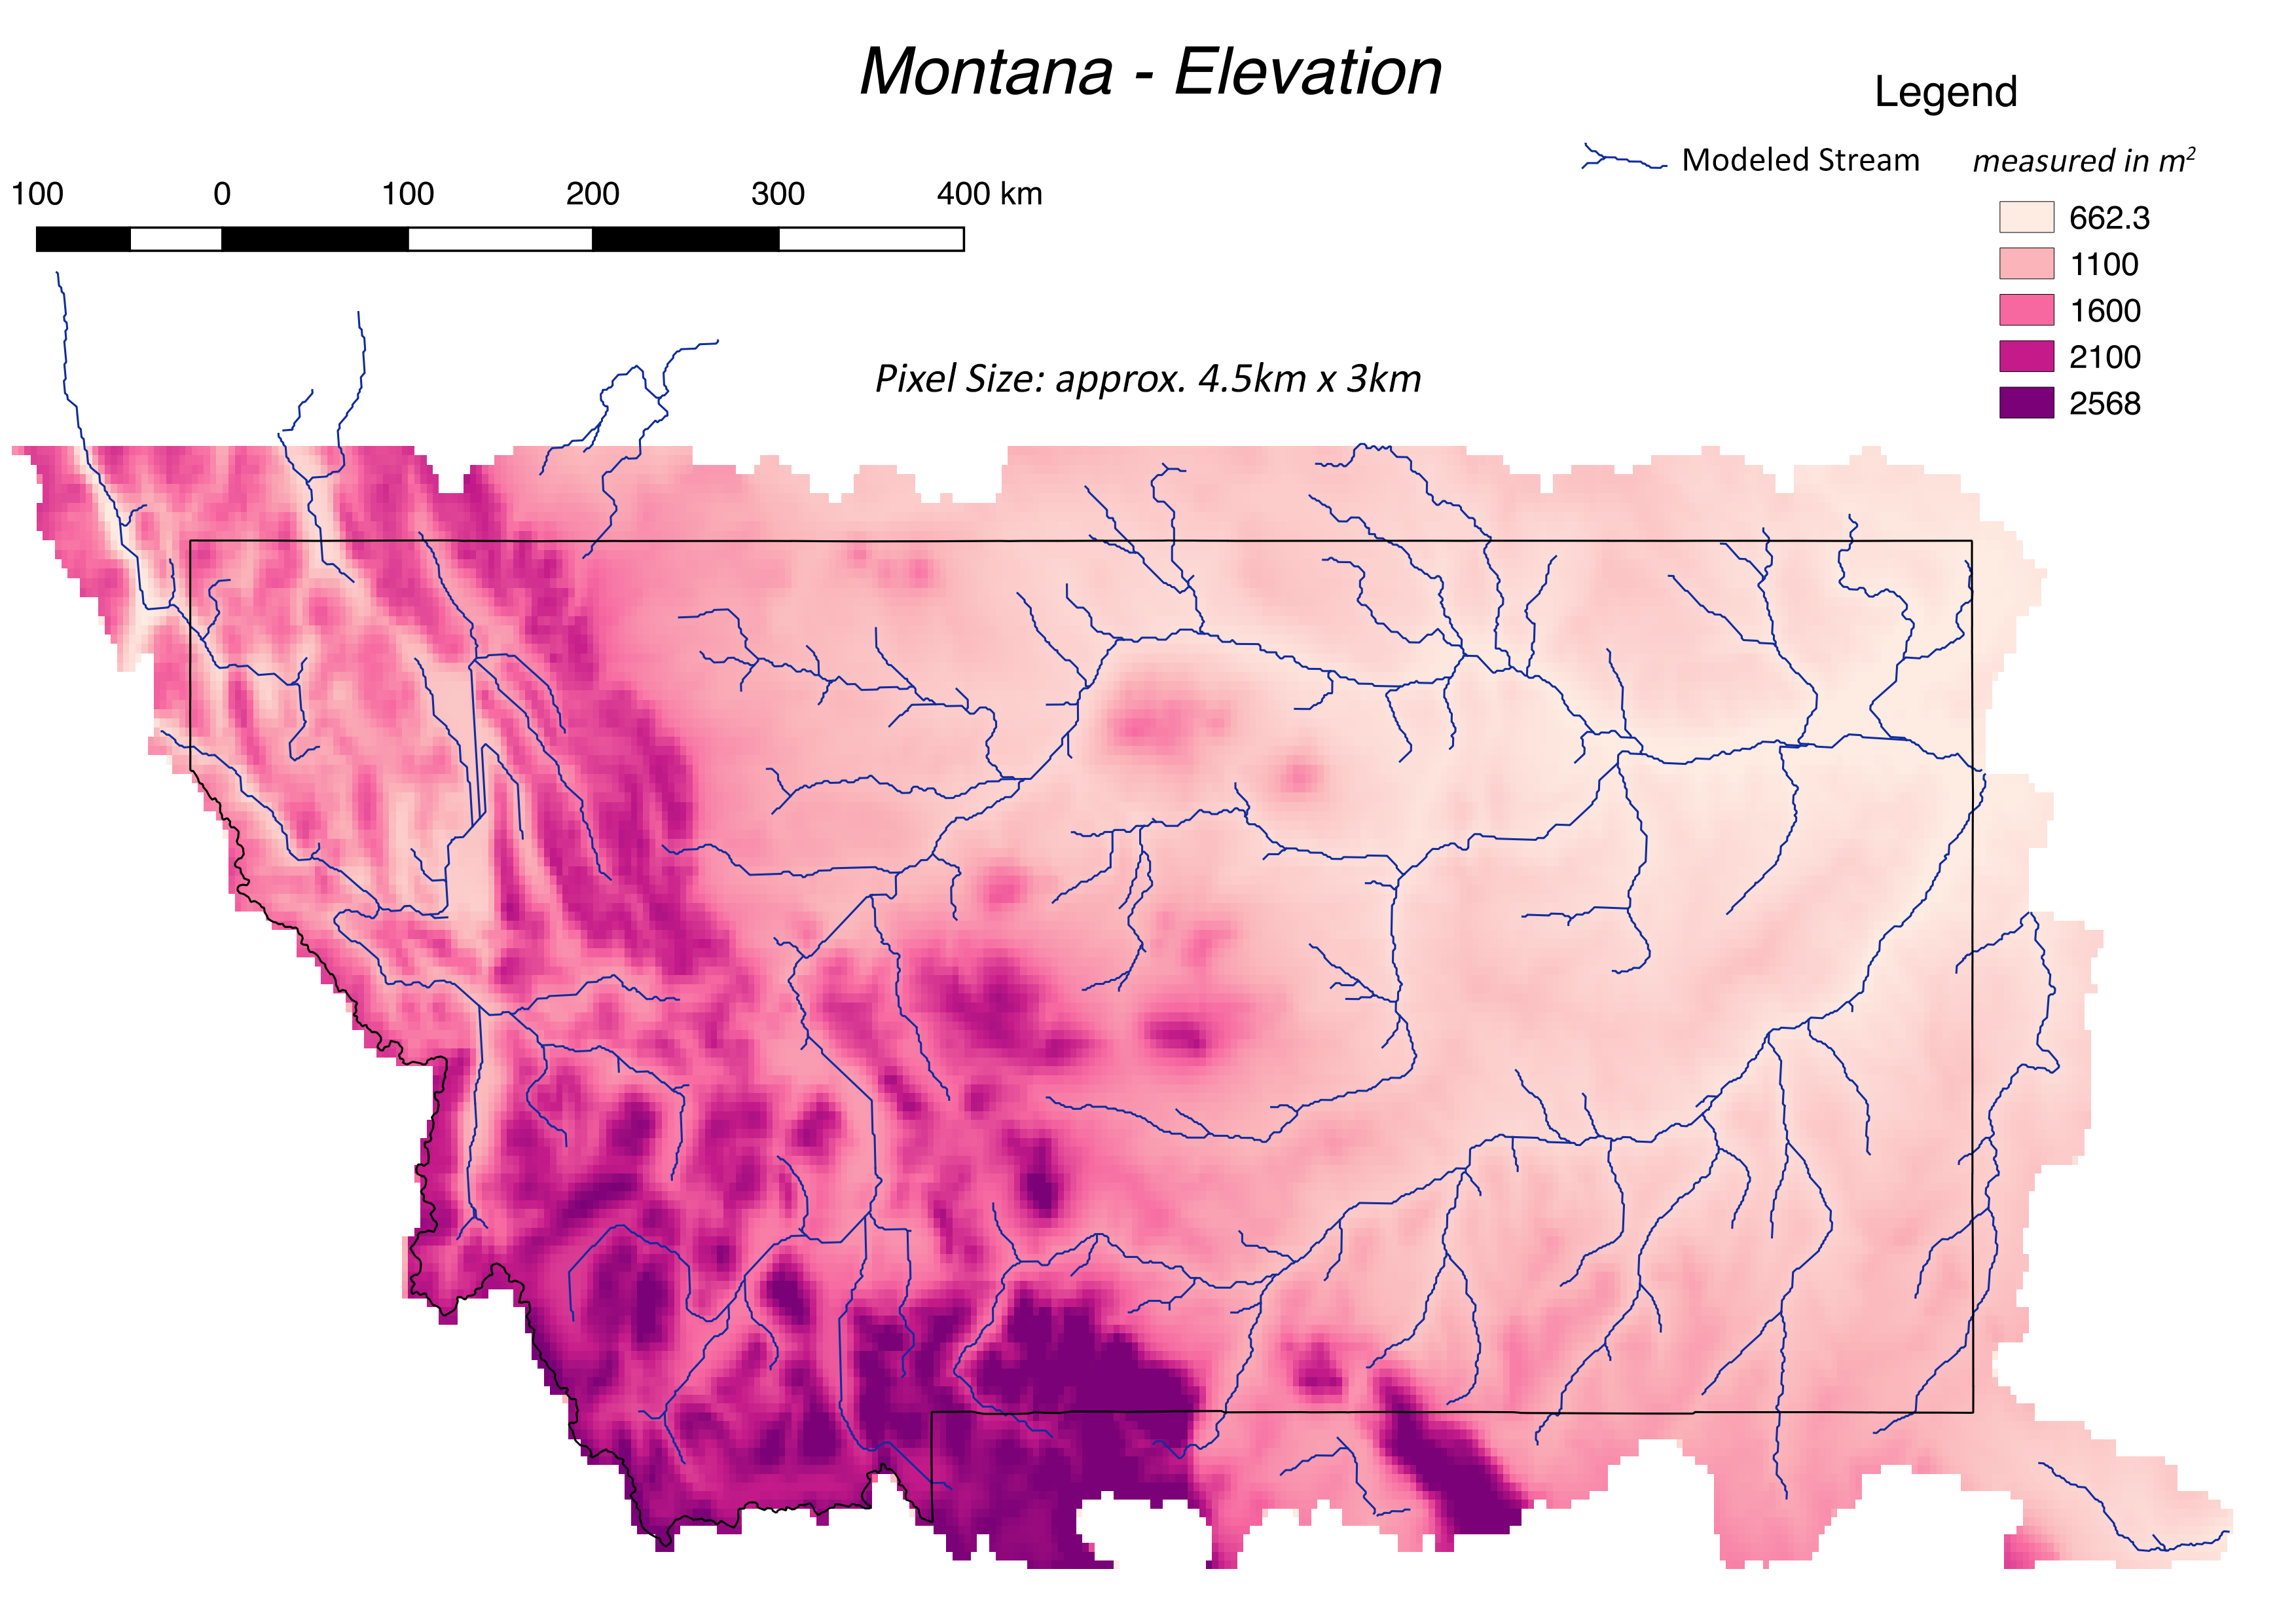
\includegraphics[width=0.95\textwidth]{elevation}
    \caption{Elevation throughout Montana}
    \label{fig:elevation}
\end{figure}

\section{Observation Data}

A Kalman Filter relies on one or more observed states for correction. Accordingly, observations were obtained for streamflows across Montana and snowfall across Montana. For streamflow, USGS streamflow data was collected at 86 sites. Each observed site was paired with the closest simulated \textbf{daWUAPhydroengine} stream outlet within a 2.5 mile cutoff. For snowfall, SNOWTEL sites monitored by the Natural Resources Conservation Service (NRCS) were used. 90 stations were chosen and matched to specific pixels in \textbf{daWUAPhydroengine}'s raster files.


\begin{table}[]
\caption{Observations} 
\begin{tabular}{lll}
Observed State ($x$) & Source                              & Dimensions  \\ \hline
streamflow  & USGS & 82   \\
swe         & NRCS & 90
\end{tabular}
\label{tab:obs}
\end{table}

\begin{figure}[h]
    \centering
    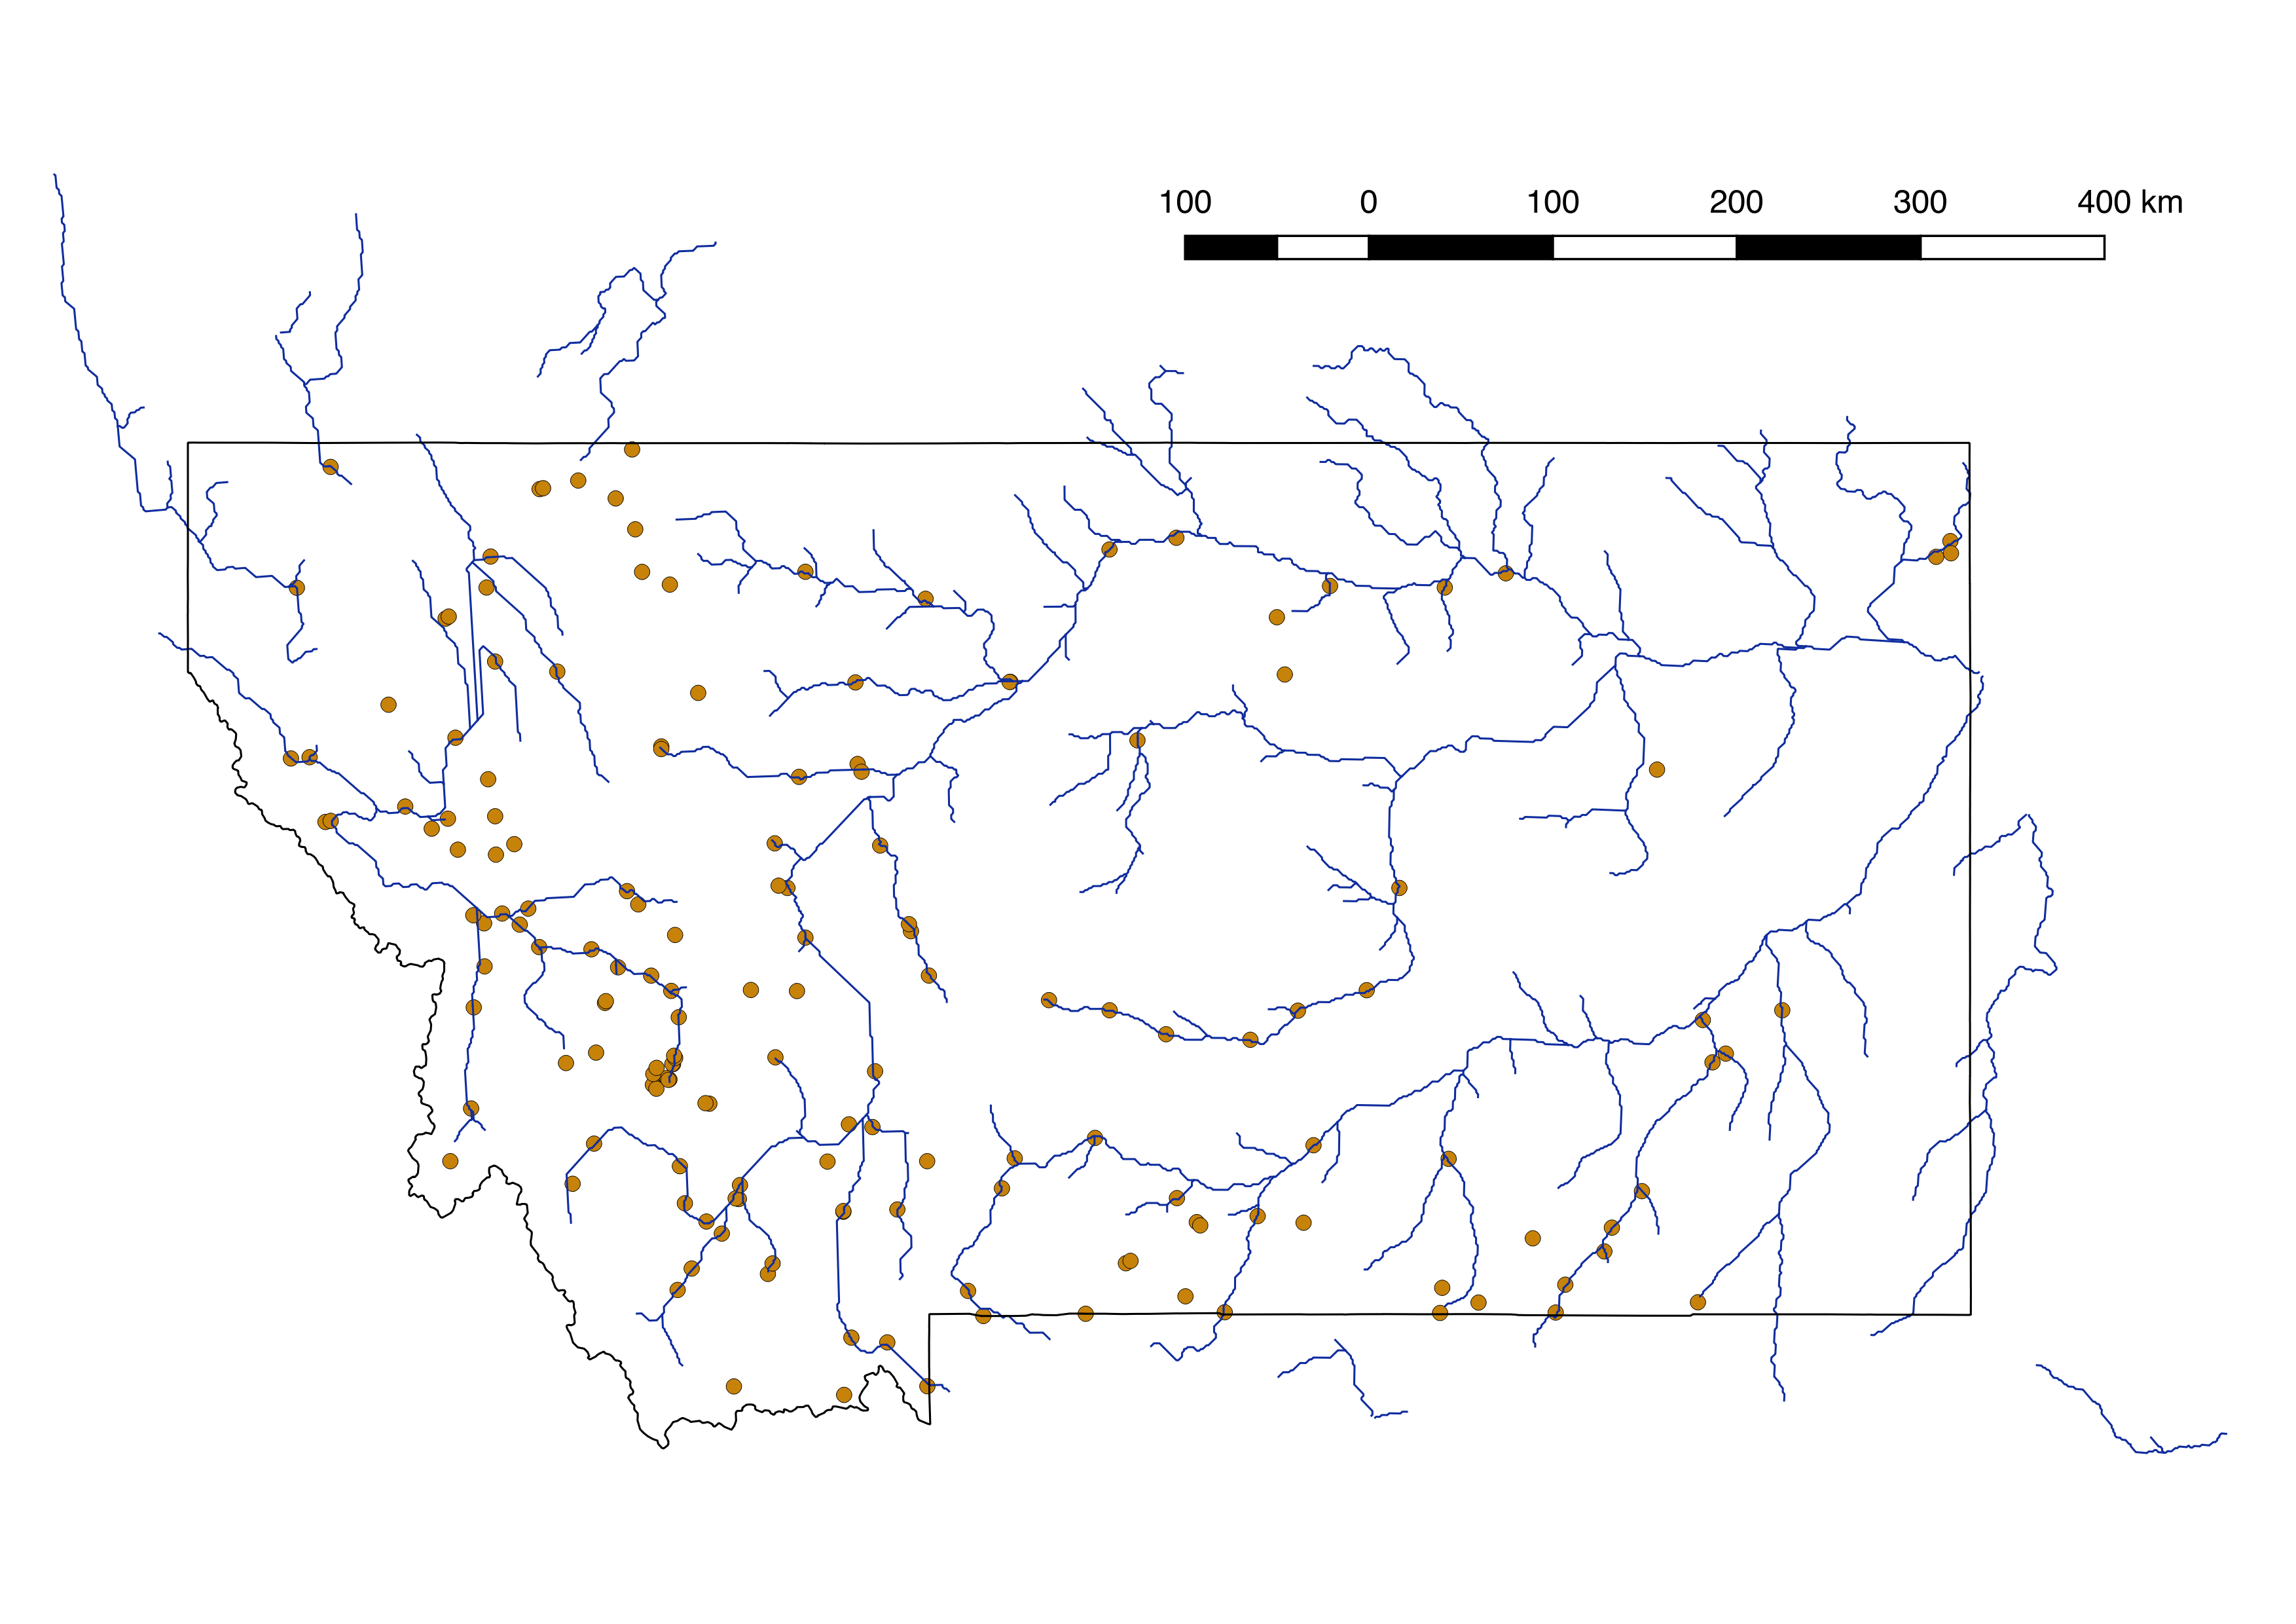
\includegraphics[width=0.95\textwidth]{stations}
    \caption{all SWE stations plotted against modeled streamflows}
    \label{fig:stations}
\end{figure}

\appendix
%% This is an example first chapter.  You should put chapter/appendix that you
%% write into a separate file, and add a line \include{yourfilename} to
%% main.tex, where `yourfilename.tex' is the name of the chapter/appendix file.
%% You can process specific files by typing their names in at the 
%% \files=
%% prompt when you run the file main.tex through LaTeX.
\chapter{The Dual Ensemble Kalman Filter}
\label{chap:dekf}

\subsection{Prediction Phase}

In a Dual Ensemble Kalman filter, each ensemble member \textit{i} is represented by a stochastic model similar to \eqref{eq:gen_stoc}. The modified equation is as follows:

\begin{equation}\label{eq:dekf_predict}
x_{t+1}^{i-} = f(x_{t}^{i+}, u_{t}^{i}, \theta^{i-}_{t}) + \omega_{t}, \quad i=1,...,n
\end{equation}

Where $n$ is the total number of ensembles. The $-/+$ superscripts denote corrected ($+$) and uncorrected ($-$) values. Note that $\theta^{i-}_{t}$'s $t$ superscript does not necessarily denote that $\theta$ is time variant but rather indicates that parameter values change as they are filtered over time. The noise term $\omega_{t}$ accounts for model error and will hereafter be excluded from the state equation.

Errors in the forcing data are accounted for through the perturbation the forcing data vector $u_{t}$ with random noise $\zeta_{t}^{i}$ to generate a unique variable $u_{t}^{i}$ for each ensemble. $\zeta_{t}^{i}$ is drawn from a normal distribution with a covarience matrix $Q_{t}^{i}$.

\begin{equation}\label{eq:dekf_u}
u_{t+1}^{i} = u_{t} + \zeta_{t}^{i}, \quad \zeta_{t}^{i} \sim N(0,Q_{t}^{i}) 
\end{equation}

To generate the priori parameters $\theta^{i-}_{t+1}$ an evolution of the parameters similar to the evolution of the state variables must be implemented. To accomplish this the kernel smoothing technique developed by West \cite{West1993} and implemented by Liu \cite{Liu2000} is used. Legacy implementations of parameter evolution added a small perturbation sampled from $N(0,\Sigma^{\theta}_{t})$, where $\Sigma^{\theta}_{t}$ represents the covariance matrix of $\theta$ at timestep $t$. This legacy method of evolution resulted in overly disposed parameter samples and the loss of continuity between two consecutive points in time \cite{Liu2000} \cite{Chen2008}. Kernel smoothing has been used effectively to solve this problem in previous Dual Ensemble Kalman filter implementations \cite{Moradkhani2005} and similar models \cite{Chen2008}.

\begin{equation}\label{eq:dekf_thetaminus}
\theta_{t+1}^{i-} = a\theta_{t}^{i+} + (1-a)\bar{\theta}_{t}^{+} + \tau_{t}^{i}
\end{equation}
\begin{equation}\label{eq:dekf_tau}
\tau_{t}^{i} = N(0, h^{2}V_{t})
\end{equation}
 
Where $\bar{\theta}_{t}^{+}$ is the mean of the parameters with respect to the ensembles, $V_{t} = var(\theta_{t}^{i+})$, $a$ is a shrinkage factor between (0,1) of the kernel location, and $h$ is a smoothing factor. $h$ is defined by $\sqrt{1-a1/2}$, while $a$ is generally between (.45,.49). Note that $h$ and $a$ tend to vary per model and optimal values for these parameters are generally found via experimentation  \cite{Moradkhani2005}  \cite{Anderson1999} \cite{Annan2005} \cite{Chen2008}.

\subsection{Parameter Correction Phase}

In an Ensemble Kalman Filter, observations are perturbed to reflect model error. Therefore, the variable $z_{t+1}^{i}$ is defined as follows:

\begin{equation}\label{eq:dekf_obs}
z_{t+1}^{i} = z_{t+1} + \eta_{t+1}^{i},\quad \eta_{t+1}^{i} = N(0,R_{t+1})
\end{equation}

Where $z_{t+1}$ is an observation vector defined by \eqref{eq:gen_obs} and $\eta_{t+1}^{i}$ is a random perturbation drawn from a normal distribution with covarience matrix $R_{t+1}$. A set of state predictions that can be related to the observations are generated by running the priori state vector through the function $h(.)$:

\begin{equation}\label{eq:dekf_pred}
\hat{y}_{t+1}^{i} = h(x_{t+1}^{i-}, \theta_{t+1}^{i-})
\end{equation}

The parameter update equation is similar to the update equation of the linear Kalman filter $\hat{x}^{+}_{t} = \hat{x}^{-}_{t} + K_{t}(z_{t}-H\hat{x}_{t})$. Notably,  parameters are corrected in lieu of the states:

\begin{equation}\label{eq:dekf_param_update}
\theta_{t+1}^{i+} = \theta_{t+1}^{i-} + K_{t+1}^{\theta}(z_{t+1}^{i}-\hat{y}_{t+1}^{i})
\end{equation}

To facilitate this, $K_{t+1}^{\theta}$ is defined as

\begin{equation}\label{eq:dekf_param_k}
K_{t+1}^{\theta} = \frac{\Sigma^{\theta,\hat{y}}_{t+1}}{\Sigma^{\hat{y},\hat{y}}_{t+1} + R_{t+1}}
\end{equation}

where $\Sigma^{\theta,\hat{y}}_{t+1}$ is the cross covariance of $\theta_{t+1}$ and $\hat{y}_{t+1}$, $\Sigma^{\hat{y},\hat{y}}_{t+1}$ is the covarience of $\hat{y}_{t+1}$, and $R_{t+1}$ is the observation error matrix from \eqref{eq:dekf_obs}. 

\subsection{State Correction Phase}

After $\theta_{t+1}^{i+}$ has been calculated the model is run again \eqref{eq:dekf_predict} with the $\theta_{t+1}^{i+}$ replacing $\theta_{t+1}^{i-}$.

\begin{equation}\label{eq:dekf_predict_2}
x_{t+1}^{i-} = f(x_{t}^{i+}, u_{t}^{i}, \theta^{i+}_{t}), \quad i=1,...,n
\end{equation}

After a new state vector is generated it is re-run through \eqref{eq:dekf_pred} with the new parameter vector:

\begin{equation}\label{eq:dekf_pred_2}
\hat{y}_{t+1}^{i} = h(x_{t+1}^{i-}, \theta_{t+1}^{i+})
\end{equation}

The corrected state vector is then run through the state update equation

\begin{equation}\label{eq:dekf_state_update}
x_{t+1}^{i+} = x_{t+1}^{i-} + K_{t+1}^{x}(z_{t+1}^{i}-\hat{y}_{t+1}^{i})
\end{equation}
 
\begin{equation}\label{eq:dekf_param_k}
K_{t+1}^{x} = \frac{\Sigma^{x,\hat{y}}_{t+1}}{\Sigma^{\hat{y},\hat{y}}_{t+1} + R_{t+1}}
\end{equation}

where $\Sigma^{x,\hat{y}}_{t+1}$ is the cross covariance of $x_{t+1}$ and $\hat{y}_{t+1}$.




%% This is an example first chapter.  You should put chapter/appendix that you
%% write into a separate file, and add a line \include{yourfilename} to
%% main.tex, where `yourfilename.tex' is the name of the chapter/appendix file.
%% You can process specific files by typing their names in at the 
%% \files=
%% prompt when you run the file main.tex through LaTeX.

\chapter{daWUAPhydroengine}

REWRITE THIS

The hydrologic system is simulated using a rainfall-runoff model coupled to a routing component that simulates streamflows in the regional stream network. We adapted the HBV model \cite{Bergstrom1995, Bergstrom1973} to simulate subcatchment-scale hydrologic processes (snowmelt, evapotranspiration, infiltration) and to transform precipitation into runoff and streamflow. Runoff that reaches the channel is routed through the stream network using the Muskingum-Cunge routing algorithm \cite{Chow1988}. In this appendix we provide here a description of the implementation of the algorithms.

\subsection{Rainfall Runoff component}

The HVB model \cite{Bergstrom1995, Bergstrom1973} is implemented as a mixture of gridded and vector-based operations to leverage the distributed nature of raster meteorological datasets while simultaneously taking advantage of the reduced computational burden of operating over polygons that aggregate runoff production over uniform hydrologic response units (HRUs).

Snowpack accumulation and melt and soil processes are calculated over the uniform raster grid imposed by the meteorological inputs (precipitation, air temperature, and potential evapotranspiration). In the next two paragraphs subscript $i$ indicates that the variable or parameter is spatially distributed and is represented at grid point $i$. Superscript $t$ indicates that the variable is dynamic and its value is represented at time step $t$. Variables with no script or superscript indicate that the variable is spatially constant or time invariant.

\paragraph{Precipitation and snowpack processes}     


Precipitation is partitioned between snowfall and rainfall using minimum and maximum daily air temperatures and a critical temperature threshold $Tc$ that determines the the snow-rain transition:

\begin{align}
Snow_i^t &= \left\{
        \begin{array}{ll}
        P_i^t &  Tmax_i^t < Tc_i \\  
        P_i^t * \frac{Tc_i - Tmin_i^t}{Tmax_i^t - Tmin_i^t} & Tmin_i^t < Tc_i < Tmax_i^t \\
        0 &  Tmin_i^t > Tc_i \\
        \end{array}
\right.\\
Rain_i^t &= P_i^t - Snow_i^t     
\end{align}
\noindent where $P$ is precipitation (\si{\milli\metre\per\day}), $T_{max}$ and $T_{min}$ are maximum and minimum air temperature (\si{\degreeCelsius}), $Rain$ is liquid precipitation and $Snow$ is snowfall at pixel $i$ during time step $t$ (\si{\milli\metre\per\day}). Snowfall during day $t$ contributes to the snow water equivalent ($SWE$, (\si{\milli\metre})) of the snowpack:

\begin{equation}
SWE_i^t = SWE_i^{t-1} + Snow_i^t \Delta t
\end{equation}

The snowpack melt process is simulated using a degree day factor model occurs when average air temperature exceeds a air temperature threshold ($Tm$):

\begin{align}
Melt_i^t &= ddf_i * (Tav_i^t - Tm_i)  ]\text{ for } Tav_i^t > Tm_i \\
Rain_i^t &= P_i^t - Snow_i^t     
\end{align}

\noindent where $Melt$ is the amount of water output from the snowpack (\si{\milli\metre\per\day}), $Tav$ is average air temperature over the time step (\si{\degreeCelsius}), and $ddf$ is the degree day factor (\si{\milli\metre\per\day\per\degreeCelsius}), an empirical parameter that represents the snowmelt rate per degree of air temperature above $Tm$. Any melt form the snowpack during time $t$ is subtracted from the snowpack storage ($SWE$) and added to the amount of water ponded in the surface:

\begin{align}
Pond_i^t &= Pond_i^{t-1} + (Melt_i^t + Rain_i^t)\Delta t \\
SWE_i^t &= SWE_i^t - Melt_i^t \Delta t   
\end{align}

\noindent where $Pond$ (\si{\milli\metre}) is liquid water available on the surface to infiltrate or produce runoff.

\paragraph{Soil processes} 
Recharge into the soil system occurs when liquid water ponding the surface infiltrates into the soil. Ponded water that is not infiltrated increases the topsoil compartment that generates fast runoff. The fraction of ponded water that infiltrates into the soil is a exponential function of the relative water storage in the soil:

\begin{align}
\Delta SM_i^t &= Pond_i^t * \left(1 - \frac{SM_i^t}{FC_i^t} \right)^\beta \\
\end{align}

\noindent where $SM$ (\si{\milli\metre}) is the amount of water in the soil compartment, $FC$ (\si{\milli\metre}) is the maximum amount of water soil can hold before water starts percolating to the groundwater system, and $beta$ (dimensionless) is an empirical parameter. Simultaneously, actual evapotranspiration ($AET$, \si{\milli\metre\per\day}) reduces the amount of water storage in the soil and is also controlled by the degree of saturation of the soil (ration of $SM$ to $FC$).

\begin{align}
AET_i^t &= PET_i^t * \left(\frac{SM_i^t}{FC_i * LP_i} \right)^l  \\
\end{align}

\noindent where $PET$ is potential evapotranspiration (\si{\milli\metre\per\day})) and $l$ is an empirical dimensionless parameter. Infiltration and actual evapotranspiration control the dynamics of water storage in the soil and amount of surface water that generates fast runoff:

\begin{align}
SM_i^t &= SM_i^{t} + \Delta SM_i^t - AET_i^t \Delta t\\
OVL_i^t &= Pond_i^t - \Delta SM_i^t
\end{align}

\noindent where $OVL$ (\si{\milli\metre}) is water that recharges the upper (near-surface) runoff-generating compartment.

\paragraph{Percolation and runoff generation}
Excess water in the topsoil and in two groundwater compartments generate outflow that represent fast and intermediate runoff and baseflow. These processes are implemented at the HRU level. For this, calculations about overland flow generation and soil moisture performed at the grid level are averaged over subwatersheds representing HRUs. Spatial arithmetic averaging soil water storage over all grid cells $i$ contained within a given HRU $j$ is represented using angle brackets $<.>$. The mass balance and percolation of water from the soil upper to the soil lower zone is implemented as:

\begin{align}
Rech_j^t &= <OVL_i^t>_j + <max(SM_i^t - FC_i, 0)>_j\\
SUZ_j^t &= SUZ_j^{t-1} + Rech_j^t + Pond_j^t - Q0_j^t\Delta t - Q1_j\Delta t - PERC_j\\
SLZ_j^t &= SLZ_j^{t-1} + PERC_j - Q2 \Delta t
\end{align}

\noindent $Rech$ (\si{\milli\meter}) is water storage in the near-surface compartment that generates fast runoff, $SUZ$ (\si{\milli\meter}) is the storage in the upper groundwater compartment, and $SLZ$ (\si{\milli\meter}) is water storage in the lower (deeper) groundwater compartment in HRU $j$ at time step $t$. $Q_0$, $Q_1$, and $Q_2$ (\si{\milli\meter\per\day}) are specific runoff rates from the soil surface, and the upper and lower soil zones:

\begin{align}
Q0_j^t &= max((SUZ_j - HL1_j) * \frac{1}{CK0_j}, 0.0)\\
Q1_j^t &= SUZ_j * \frac{1}{CK1_j}\\
Q2_j^t &= SLZ_j * \frac{1}{CK2_j}\\
Qall_j^t &= Q0_j^t + Q1_j^t + Q2_j^t
\end{align}

\noindent where $HL1$ (\si{\milli\meter}) is an empirical water storage threshold the triggers the generation of fast runoff, and $CK0$, $C10$, $CK2$ (\si{\day}) are empirical parameters representing the characteristic drainage time of each of the compartments.
Total outflow from HRU $j$ on day $t$ is distributed over time to produce the catchment response by convoluting the output of HRU $j$ by triangular standard unit hydrograph with base $M_{base}$.

\begin{align}
Q_j^t &= \sum_{i=1}^{M_{base}} Qall_j^{t-i+1} U(i) \\
U(i) &= \left\{
\begin{array}{ll}
\frac{4}{M_{base}^2}*i & 0 < i < M_{base}/2 \\
-\frac{4}{M_{base}^2}*i + \frac{4}{M_{base}} &  M_{base}/2 < i < M_{base} \\
\end{array}
\right.
\end{align}

\noindent where $U$ is a triangular hydrograph of area \num{1} and a base $MAXBAS$ (\si{\day})representing the hydrograph duration . 

\subsection{Routing component}

The response at the end of each $HRU$ is routed through the stream network using the Muskingum-Cunge routing model. In this model the storage in each stream reach $k$ is given by the following discharge-storage equation:

\begin{align}
S_k^t &= K\left[eQ_{in} + (1 - e)Q_{out} \right],
\end{align}

which has parameters $K$ (\si{\day}) and $e$ (dimensionless) controlling, respectively, the celerity and dispersion of the wave routed through the channel.

Substituting this relationship in a finite-difference form of the continuity equation $\frac{S_j^{t+1} - S_j^{t}}{\Delta t} = Q_{in} - Q_{out}$ for a multi-reach system with lateral inflows injected upstream of reach draining $HRU$ $j$ at average constant rate through time step $t$ $q_{j}^{t+1}$ yields:

\begin{align}
&Q_j^{t+1}\left[K_j(1 - e_j) + 0.5\Delta t  \right] + Q_{j-1}^{t+1}\left[K_je_j - 0.5\Delta t  \right]  \\
&= Q_j^{t}\left[K_j(1 - e_j) - 0.5\Delta t  \right] + Q_{j-1}^{t}\left[K_je_j + 0.5\Delta t  \right]\\
&+ q_{j}^{t+1}\left[K_j(1 - e_j) + 0.5\Delta t  \right]
\end{align}

Each of the $HRUs$ contains one reach with an upstream and a downstream node. Streamflows for each of the $j=1,...,J$ reaches are integrated over time using a first-order explicit finite difference scheme. The system of $J$ equations can be assembled as a linear system of the form:   

\begin{align}\label{eq:linearsystem}
\mathbf{A}\mathbf{Q^{t+1}} = \mathbf{B}
\end{align}

where $\mathbf{Q^{t+1}}$ is the vector of unknown streamflows at time $t+1$ for each of the $J$ reaches of the network that is solved each time step. Matrices $\mathbf{A}$ add $\mathbf{B}$ are functions of the model parameters and streamflows at timestep $t$:
\begin{align}
\mathbf{A}&\equiv (\mathbf{a} + \mathbf{\Phi} \mathbf{b})^T\\
\mathbf{B}&\equiv (\mathbf{d} + \mathbf{\Phi}\mathbf{c})^T\mathbf{Q}^t + \mathbf{I}(\mathbf{a\odot q}^{t+1})
\end{align}

where $\mathbf{\Phi}$ is a $JxJ$ sparse connectivity (0,1)-matrix where the elements indicate if two pairs of nodes are connected. Flow direction is from nodes in the rows to nodes in the columns. Rows representing the upstream node of $HRUs$ that drain an outlet node (exit the domain) are all zero. Finally,

%\begin{align}
%(\mathbf{a} + \mathbf{\Phi} \mathbf{b})\mathbf{Q^{t+1}} = (\mathbf{d} + %\mathbf{\Phi}\mathbf{c})\mathbf{Q^t} + \diag(\mathbf{a})*\mathbf{q^{t+1}}
%\end{align}

\begin{align}
\mathbf{a} &= \mathbf{I} (\mathbf{K}-\mathbf{K\odot e}) + dt * 0.5\\
\mathbf{b} &= \mathbf{I} (\mathbf{K\odot e}) - dt * 0.5\\
\mathbf{c} &= \mathbf{I} (\mathbf{K}-\mathbf{K\odot e}) - dt * 0.5)\\
\mathbf{d} &= \mathbf{I} (\mathbf{K\odot e}) + dt * 0.5
\end{align}

\noindent where $\mathbf{K}$ is the identity matrix of order $J$, $\mathbf{K}$ and $\mathbf{e}$ are column vectors holding parameters $K$ and $e$ for each of the $N$ reaches in the network. The $\odot$ operator denotes the Schur (elementwise) product between two vectors.
The solution of \eqref{eq:linearsystem} becomes unstable if $\Delta t > 2 * K_j * (1 - e_j)$. To ensure robust and stable solution an adaptive time stepping scheme was implemented. In this scheme, the default time step is reduced by an integer fraction until the the stability condition is satisfied in all reaches. 




%% This defines the bibliography file (main.bib) and the bibliography style.
%% If you want to create a bibliography file by hand, change the contents of
%% this file to a `thebibliography' environment.  For more information 
%% see section 4.3 of the LaTeX manual.
\begin{singlespace}
\bibliography{main}
\bibliographystyle{plain}
\end{singlespace}

\end{document}

